% Created 2021-08-17 Di 11:51
% Intended LaTeX compiler: pdflatex
\documentclass[11pt]{article}
\usepackage[utf8]{inputenc}
\usepackage[T1]{fontenc}
\usepackage{graphicx}
\usepackage{grffile}
\usepackage{longtable}
\usepackage{wrapfig}
\usepackage{rotating}
\usepackage[normalem]{ulem}
\usepackage{amsmath}
\usepackage{textcomp}
\usepackage{amssymb}
\usepackage{capt-of}
\usepackage{hyperref}
\author{Marcus Birkenkrahe}
\date{\today}
\title{Course overview\\\medskip
\large Data modeling}
\hypersetup{
 pdfauthor={Marcus Birkenkrahe},
 pdftitle={Course overview},
 pdfkeywords={},
 pdfsubject={},
 pdfcreator={Emacs 27.2 (Org mode 9.3.7)}, 
 pdflang={English}}
\begin{document}

\maketitle
\section*{What're you going to learn today?}
\label{sec:org1ca8995}

\begin{itemize}
\item Who is your lecturer?
\item Who are you and what do you want?
\item Which topics will we cover?
\item How will we do it?
\item What do you have to do to pass?
\item What's next?
\end{itemize}

\section*{Who am I?}
\label{sec:orge9cf6cd}

\begin{center}
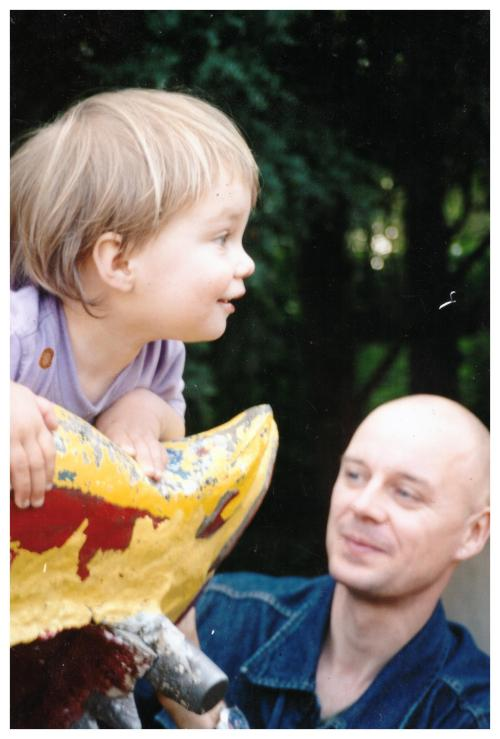
\includegraphics[width=.9\linewidth]{./img/marcus.jpg}
\end{center}

\subsection*{Science}
\label{sec:orgb911ab2}

\begin{center}
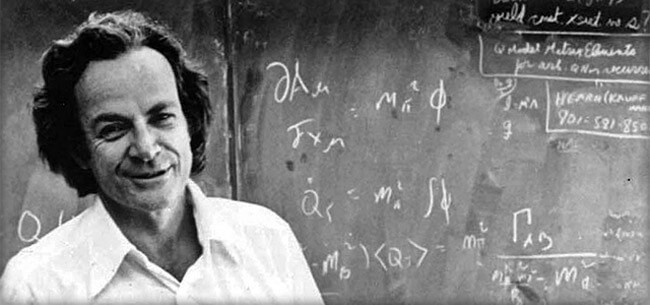
\includegraphics[width=300px]{./img/feynman.jpg}
\end{center}

\begin{itemize}
\item Development of WWW
\item PhD theoretical particle physics
\item 60 research publications
\item Assoc. Ed. Int. J. of Data Science
\item Ed. Board Int. J. of Big Data Mgmt.
\item Scientific member \href{https://www.hwr-berlin.de/en/research/research-centres-and-institutes/}{d-cube@Berlin}
\end{itemize}

\subsection*{Industry}
\label{sec:orgfc8ff37}

\begin{center}
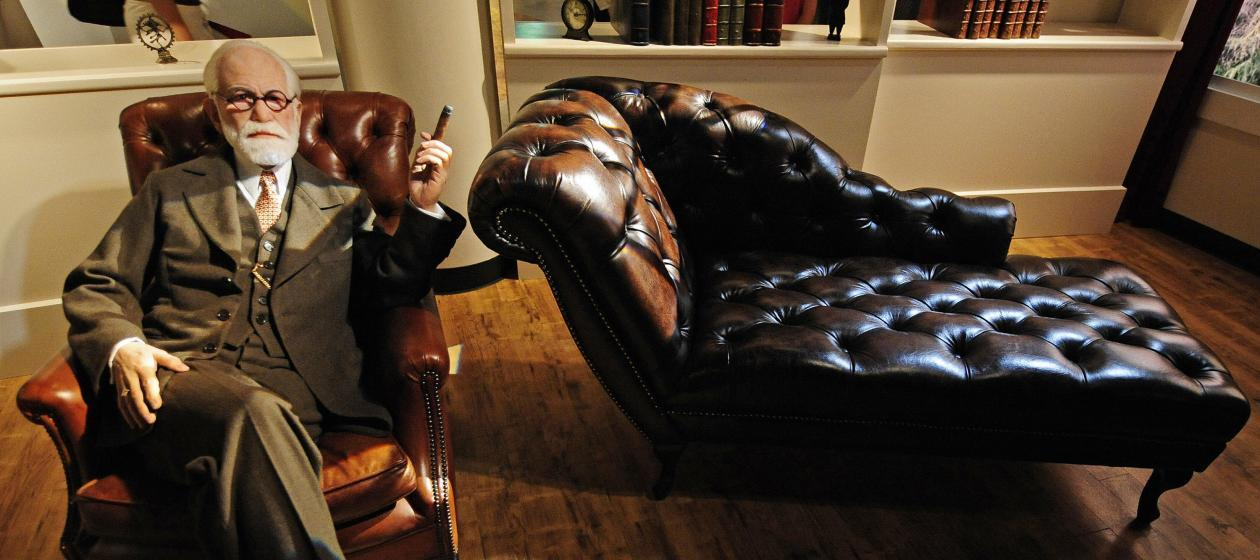
\includegraphics[width=300px]{./img/freud.jpg}
\end{center}

\begin{itemize}
\item Executive at Accenture \& Shell
\item Coach and consultant
\item Certified psychotherapist
\item Startup mentor
\end{itemize}

\subsection*{Teaching}
\label{sec:orgc101cec}

\begin{center}
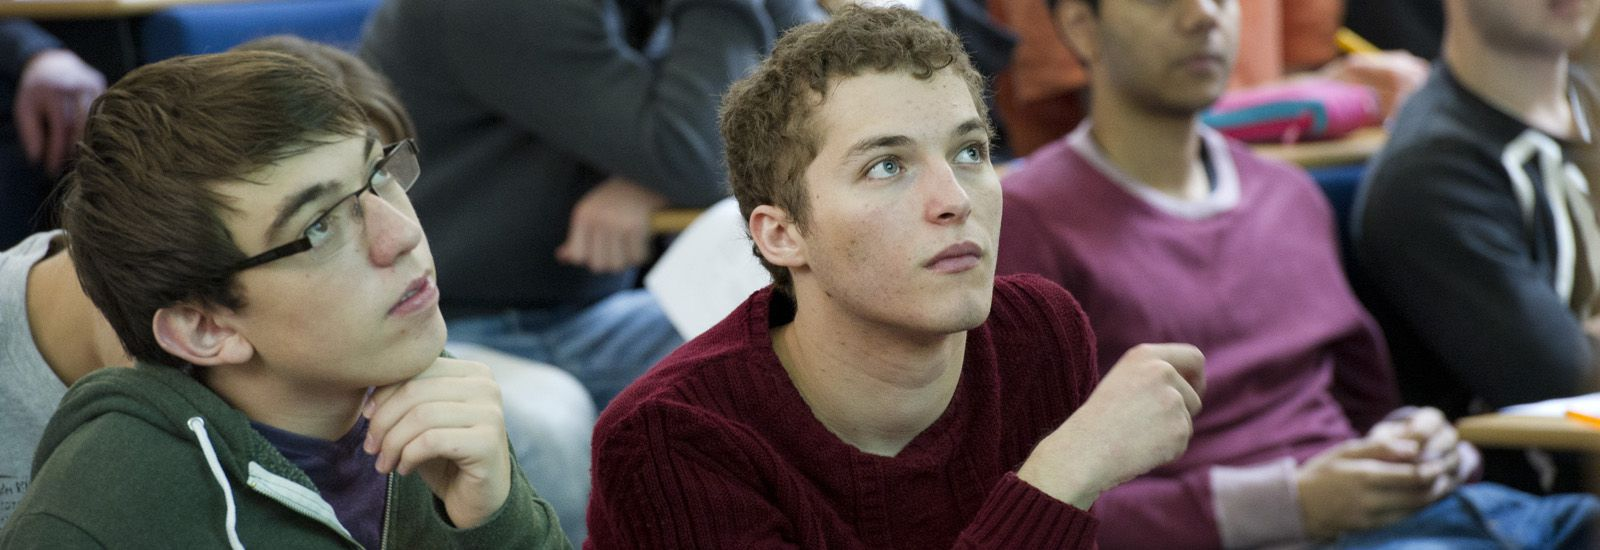
\includegraphics[width=300px]{./img/teaching.jpeg}
\end{center}

\begin{itemize}
\item Business informatics \href{https://www.hwr-berlin.de/en/}{@HWR Berlin}
\item Visiting professor of data science @Lyon
\item Adviser for \href{https://catholicpolytechnic.org/}{CPU @LA}
\item Internship supervision
\end{itemize}

\subsection*{Pleasure}
\label{sec:org1b89215}

\begin{center}
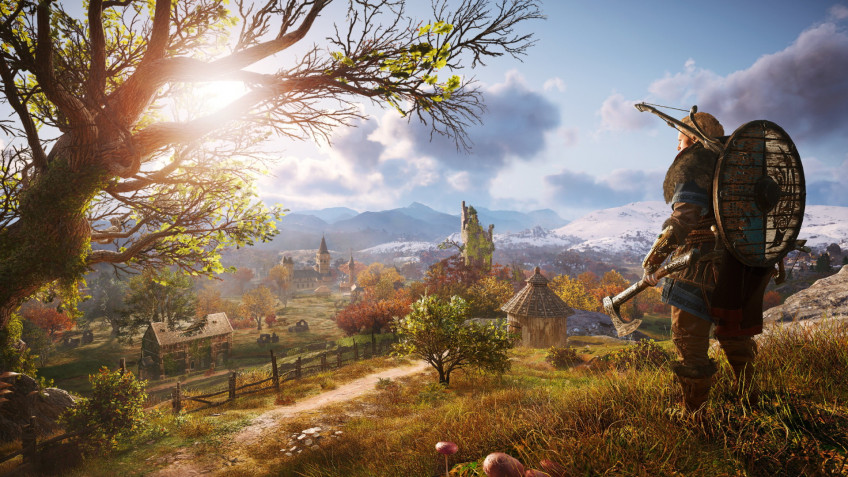
\includegraphics[width=300px]{./img/valhalla.jpg}
\end{center}

\begin{itemize}
\item Playing: \href{https://en.wikipedia.org/wiki/Assassin\%27s\_Creed\_Valhalla}{Assassin's Creed Valhalla} (2020)
\item Reading: \href{https://en.wikipedia.org/wiki/Sword\_of\_Honour}{Waugh, Sword of Honour} (1952-1961)
\item Watching: \href{https://en.wikipedia.org/wiki/The\_Middle\_(TV\_series)}{The Middle} (2009-2018)
\end{itemize}

\section*{\href{https://ideaboardz.com/for/Data\%20modeling\%20expectations/4047934}{What are your expectations?}}
\label{sec:org17238e9}

\begin{itemize}
\item What do you want to learn here?
\item What would you like to avoid?
\item What did you take away from another course?
\item What did you really not like in another course?
\end{itemize}

\section*{Which topics will we cover?}
\label{sec:org96174ca}

\url{./img/lavaflow.gif}

\subsection*{Many-model thinking}
\label{sec:org2c38e14}

\begin{center}
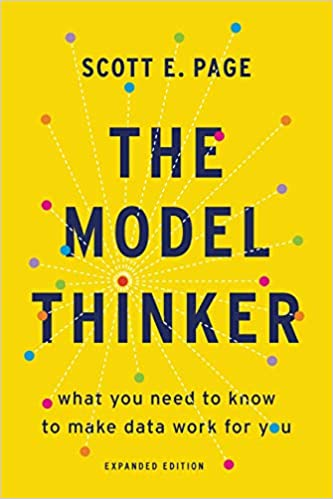
\includegraphics[width=.9\linewidth]{./img/pagebook.jpg}
\end{center}

\href{https://www.amazon.com/Model-Thinker-What-Need-Know-ebook-dp-B07B8D3V9V/dp/B07B8D3V9V/}{Expanded edition, Basic Books 2021}

\subsection*{Decision intelligence}
\label{sec:orgcce1c1a}

\begin{center}
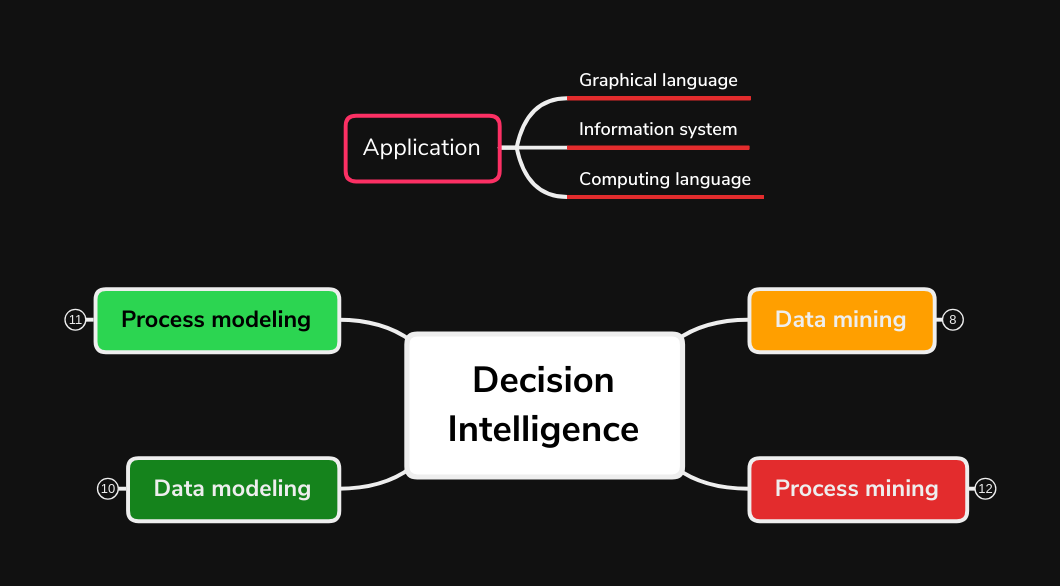
\includegraphics[width=.9\linewidth]{./img/decision_intelligence.png}
\end{center}

\subsection*{Process Modeling}
\label{sec:orgb04dd21}

\begin{center}
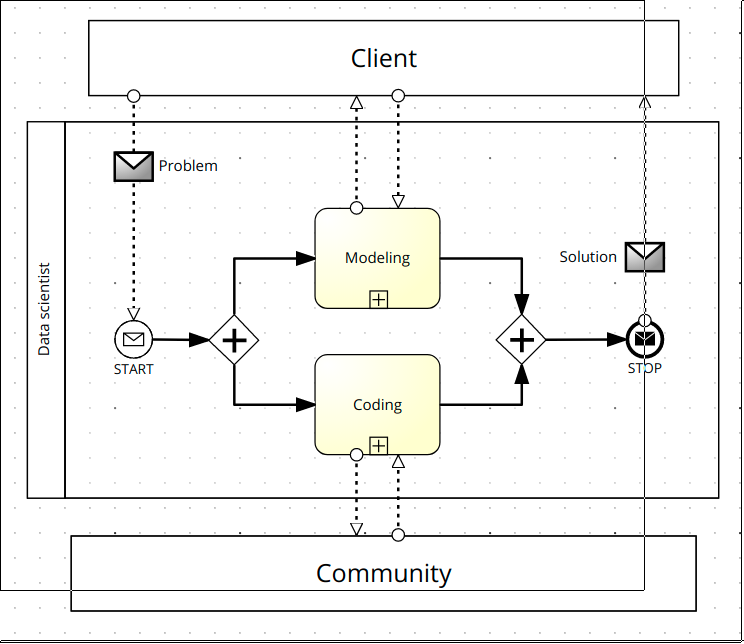
\includegraphics[width=.9\linewidth]{./img/bpmn.png}
\end{center}

Source: Signavio / 19 May test lecture

\subsection*{Linear models}
\label{sec:org954ccd8}

\begin{center}
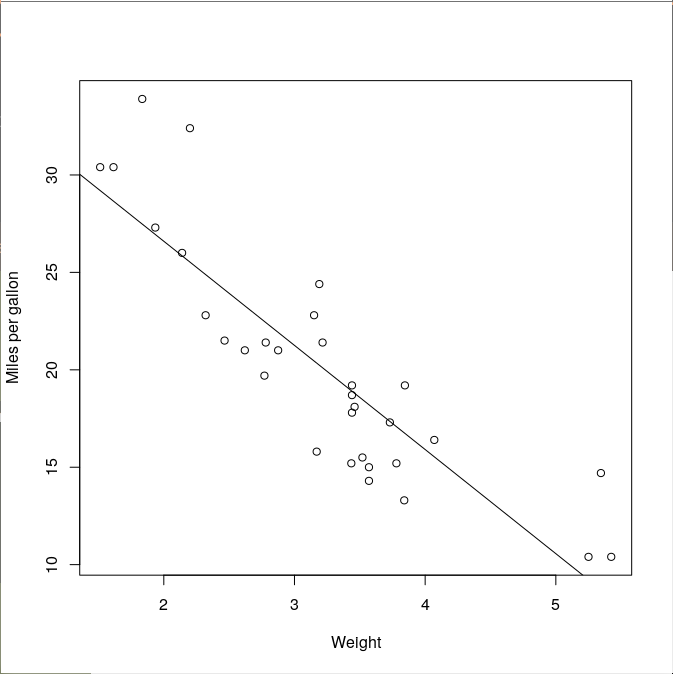
\includegraphics[width=.9\linewidth]{./img/linear.png}
\end{center}

Source: R plot
\subsubsection*{Linear regression in R}
\label{sec:org969cc9a}

\begin{verbatim}
x <- mtcars$wt
y <- mtcars$mpg
plot(x,y,xlab="Weight",ylab="Miles per gallon")
lm_model <- lm(y~x,data=mtcars)
abline(lm_model)
\end{verbatim}

\subsection*{Agile management}
\label{sec:org51f4722}

\begin{center}
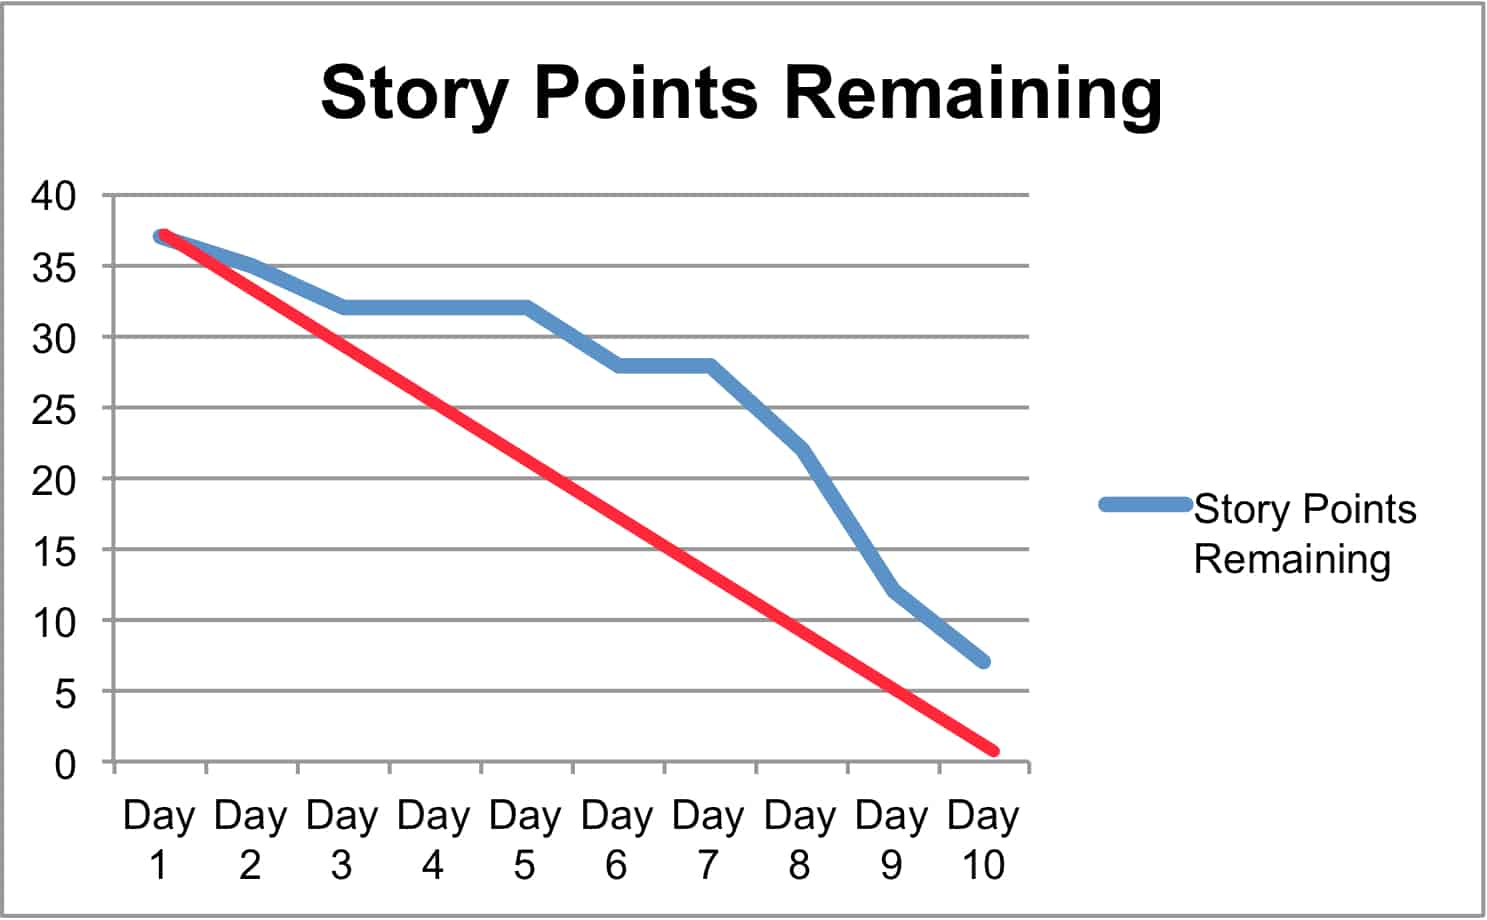
\includegraphics[width=.9\linewidth]{./img/burndown.jpg}
\end{center}

Image: \href{https://www.scrum.org/}{Scrum} burndown chart

\subsection*{Robotic Process Automation}
\label{sec:org48d8774}

\begin{center}
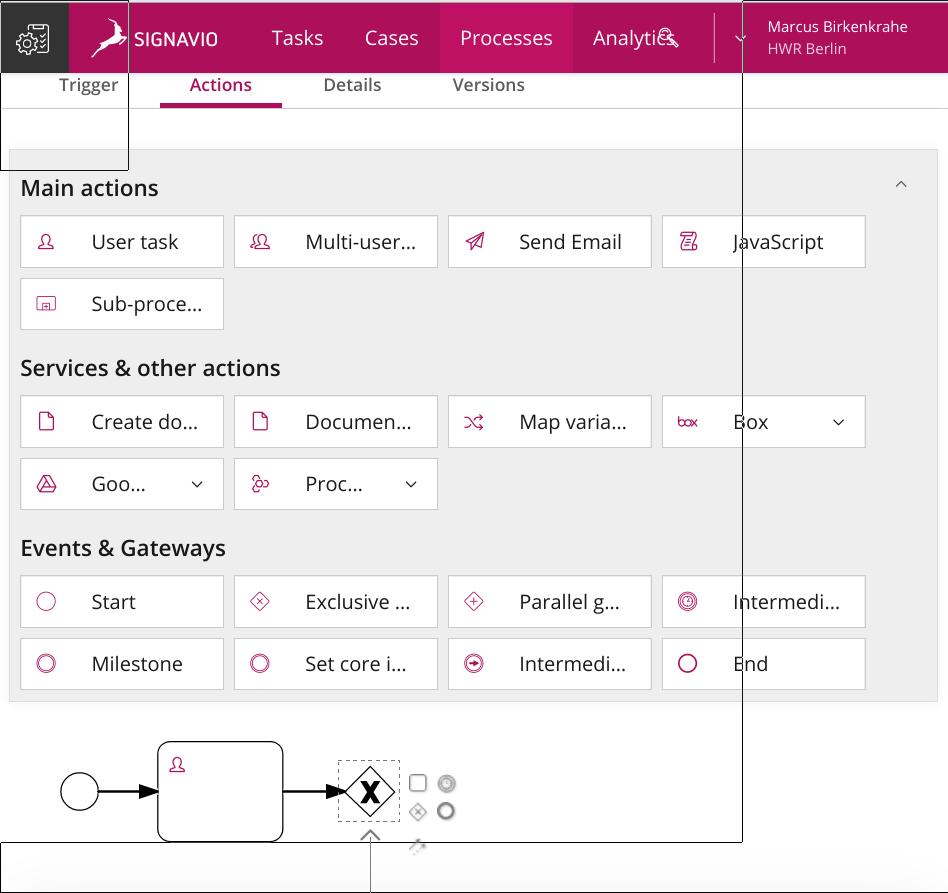
\includegraphics[width=.9\linewidth]{./img/rpa.png}
\end{center}

Image: \href{https://www.signavio.com/products/workflow-accelerator/}{Signavio Workflow Accelerator}

\subsection*{Unified Modeling Language}
\label{sec:orgb3e099f}

\begin{center}
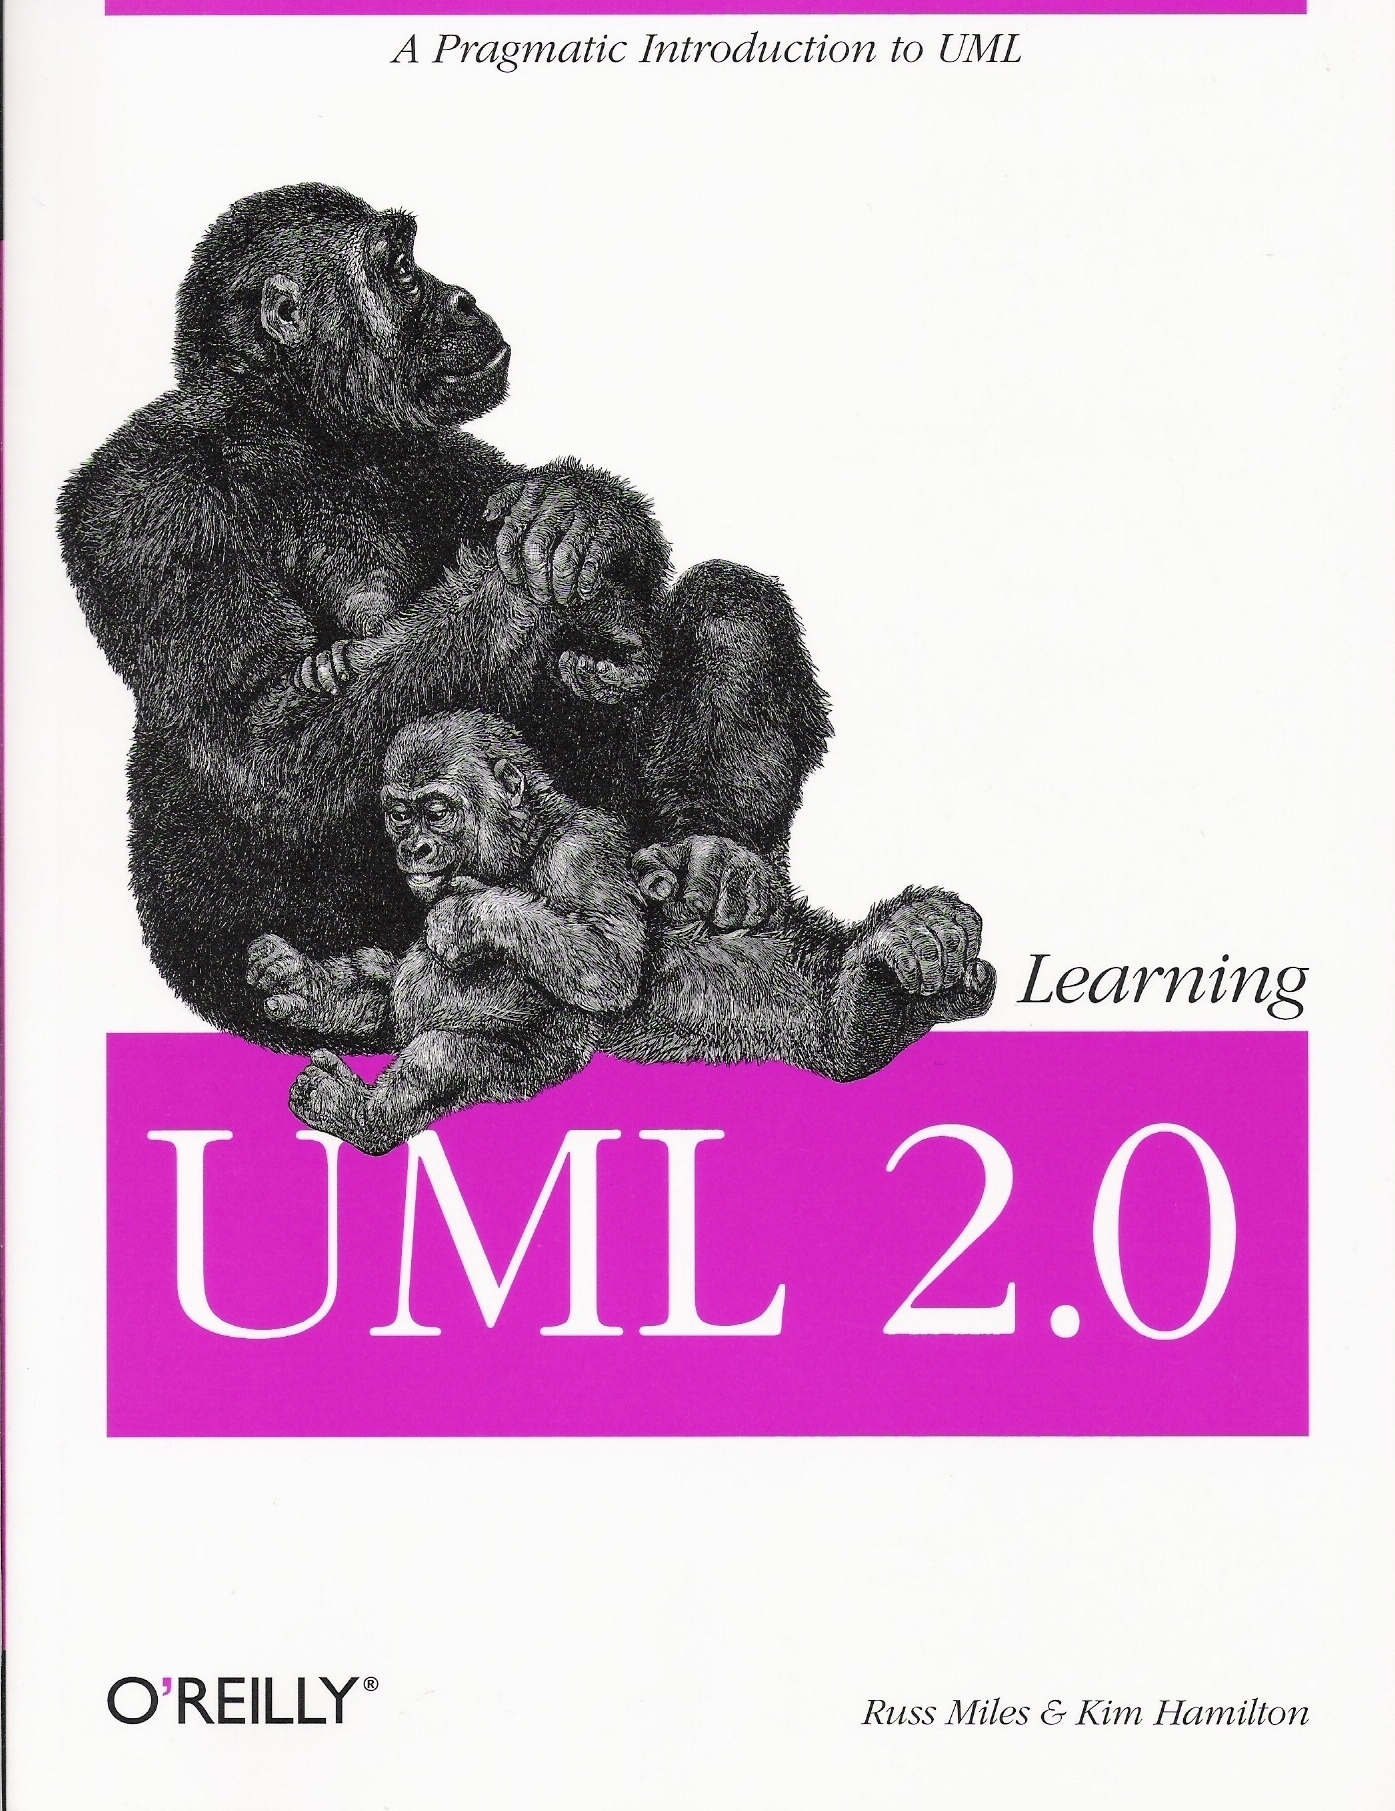
\includegraphics[width=.9\linewidth]{./img/uml.jpg}
\end{center}

Image: \href{https://www.amazon.com/Learning-UML-2-0-Pragmatic-Introduction-ebook-dp-B0028N4WII/dp/B0028N4WII/}{Learning UML 2.0} (2006)

\subsection*{Process mining}
\label{sec:org685125f}

\begin{center}
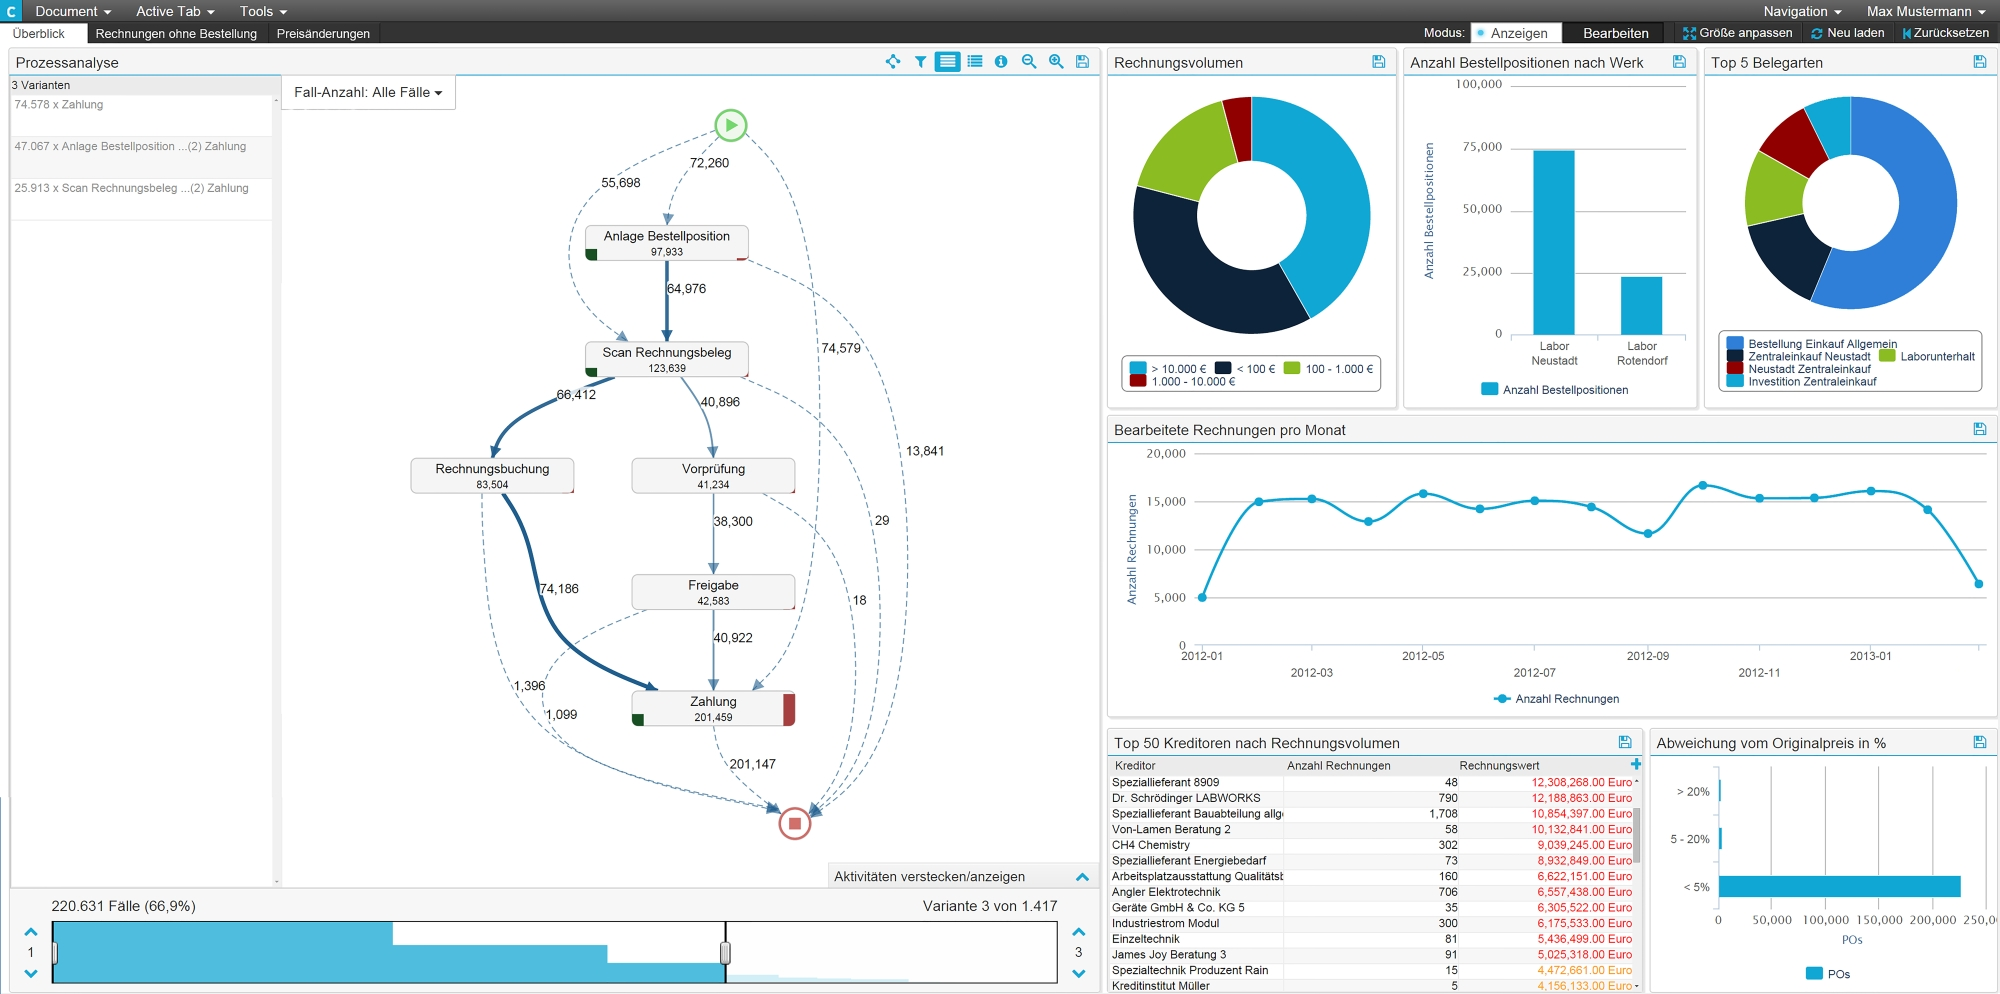
\includegraphics[width=.9\linewidth]{./img/processmining.jpg}
\end{center}

Image: \href{https://www.celonis.com/}{Celonis} dashboard

\subsection*{Schedule (see \href{https://github.com/birkenkrahe/mod482/blob/main/syllabus.md}{Syllabus})}
\label{sec:org1564940}

\begin{center}
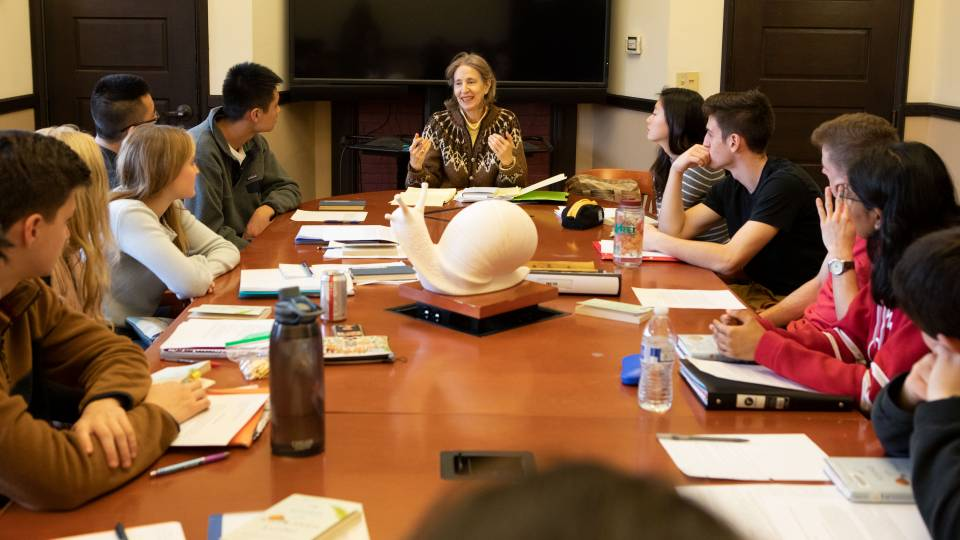
\includegraphics[width=.9\linewidth]{./img/seminar.jpg}
\end{center}

Image: \href{https://www.princeton.edu/news/2018/12/03/life-unpacked-freshman-seminar-explores-search-meaningful-life}{Princeton U.}

\section*{How will we do it?}
\label{sec:org299b909}

\url{./img/deer.gif}

\subsection*{Classroom sessions}
\label{sec:org454faf4}

\begin{center}
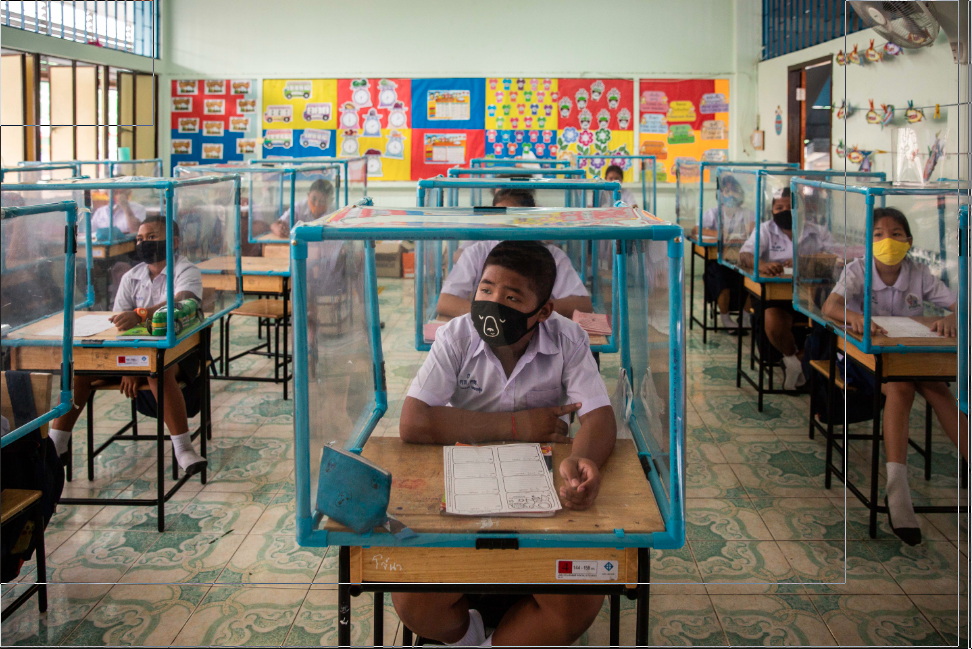
\includegraphics[width=.9\linewidth]{./img/classroom.png}
\end{center}

\subsection*{Lecture scripts with exercises (\href{https://github.com/birkenkrahe/mod482}{GitHub})}
\label{sec:orgb05dc97}

\begin{center}
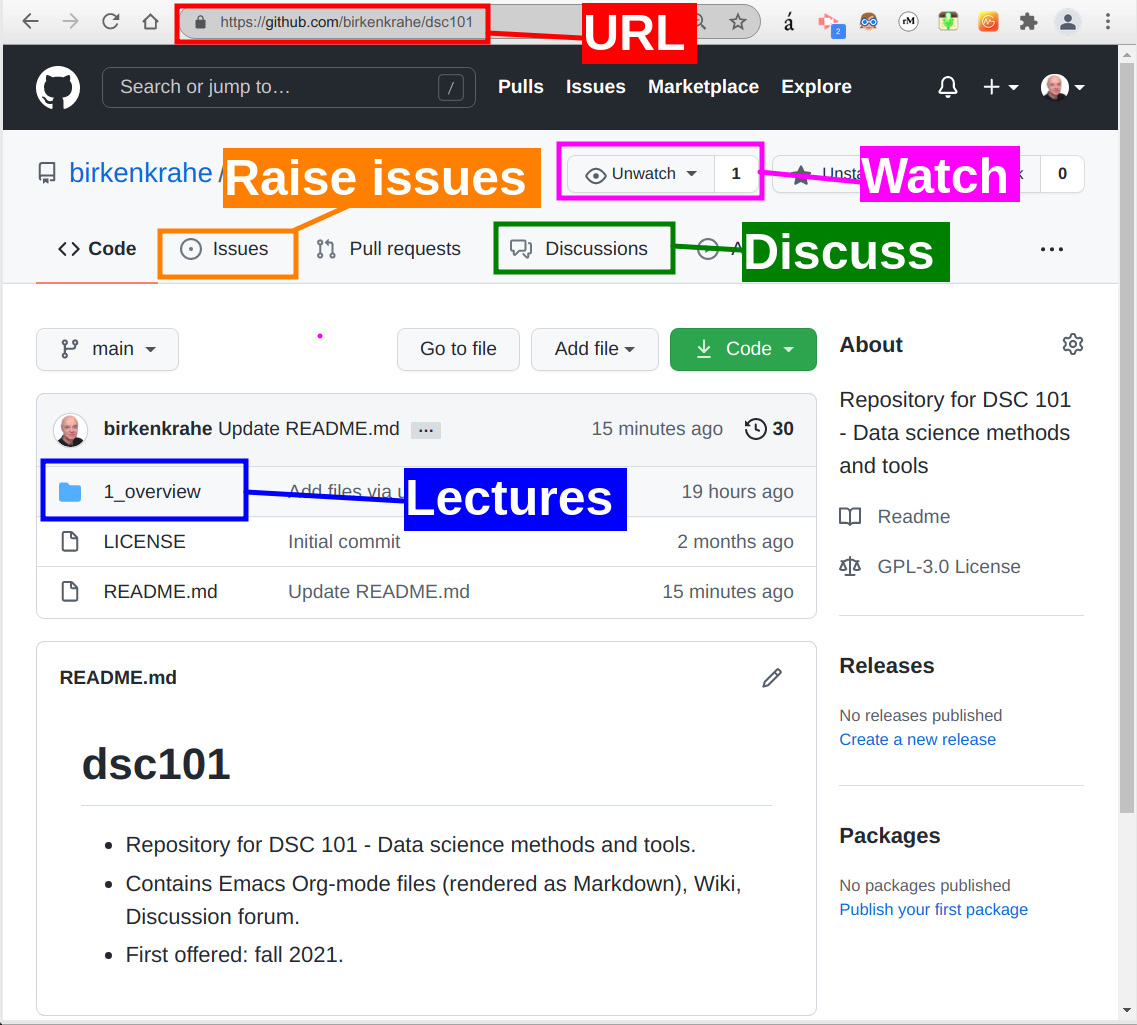
\includegraphics[width=.9\linewidth]{./img/github.png}
\end{center}

\subsection*{Reading assignments}
\label{sec:org9780c9c}

\begin{center}

\includegraphics[width=.9\linewidth]{./img/books.jpeg}
\end{center}

\begin{itemize}
\item Image: Unsplash (\href{https://unsplash.com/photos/9BoqXzEeQqM}{@tomhermans})
\end{itemize}

\subsection*{Lab sessions}
\label{sec:orgd30a45e}

\begin{center}
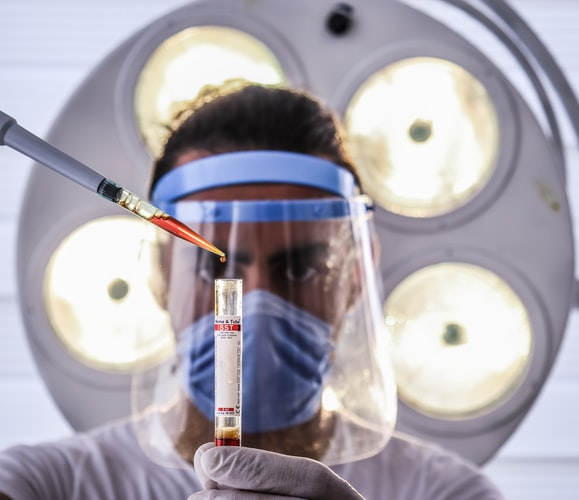
\includegraphics[width=.9\linewidth]{./img/lab.jpeg}
\end{center}

\begin{itemize}
\item Image: Unsplash (\href{https://unsplash.com/photos/MD2\_srN-02o}{@Emin Baycan})
\end{itemize}

\subsection*{Stuff you bring to class}
\label{sec:org69d5b3f}

\begin{center}
\includegraphics[width=.9\linewidth]{./img/scrapyard.jpg}
\end{center}

\begin{itemize}
\item Image: Unsplash (\href{https://unsplash.com/photos/HGCqL-tRcac}{@Evan Demicoli})
\end{itemize}

\section*{What do you have to do to pass?}
\label{sec:org0651bba}

\url{./img/oceanrock.gif}

\subsection*{Weekly lab practice (> 50\%)}
\label{sec:org6e0af14}

\begin{center}
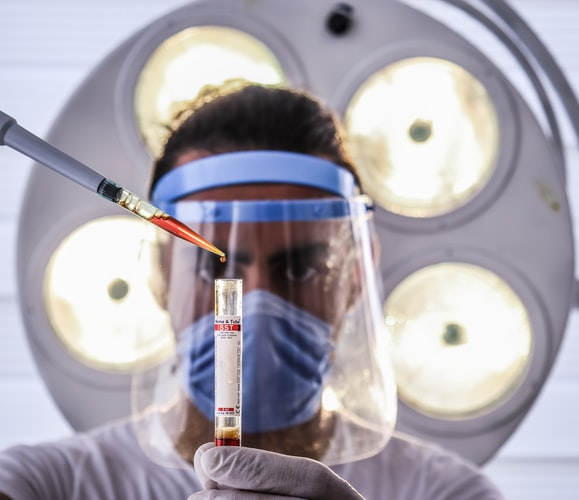
\includegraphics[width=.9\linewidth]{./img/lab.jpeg}
\end{center}

\subsection*{Weekly participation (> 50\%)}
\label{sec:org8730331}

\begin{center}
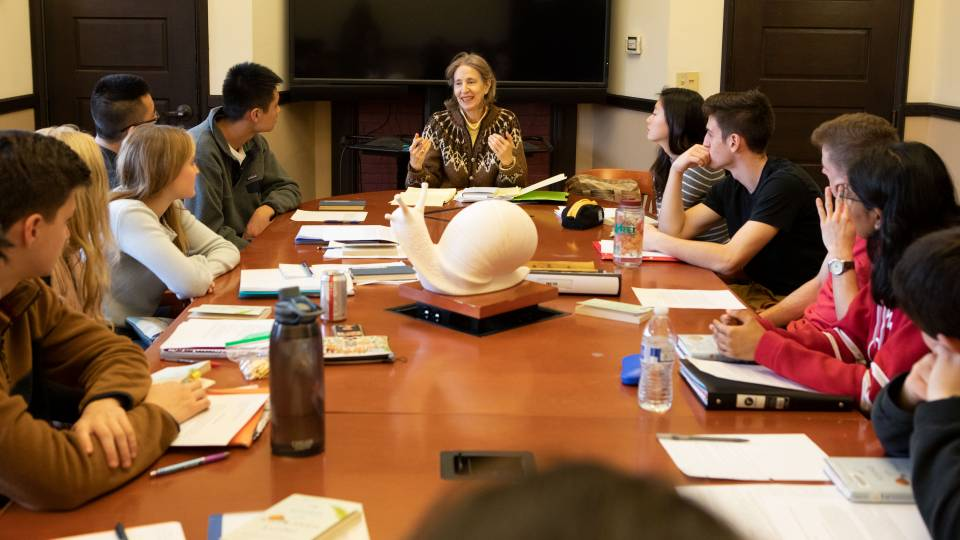
\includegraphics[width=.9\linewidth]{./img/seminar.jpg}
\end{center}

\subsection*{Final essay (> 50\%)}
\label{sec:orgdc37e26}

\begin{center}

\includegraphics[width=.9\linewidth]{./img/essay.jpg}
\end{center}

Source: Unsplash (\href{https://unsplash.com/photos/y02jEX\_B0O0}{@Aaron Burden})

\subsubsection*{What constitutes an essay?}
\label{sec:org38a063c}

\begin{itemize}
\item IMRaD structure (\href{https://youtu.be/dip7UwZ3wUM}{video})
\item Research question
\item Literature review
\item Methodology
\item Results (e.g. glossary)
\item Discussion with limitations
\item References
\end{itemize}

\subsubsection*{Do you have essay examples?}
\label{sec:org777388b}

\begin{itemize}
\item Chapters in "Model thinking"
\item (Parts of) Research papers
\item Scientific or industry blogs
\end{itemize}

\subsubsection*{Can I write a scientific essay?}
\label{sec:org3c882c4}

\begin{itemize}
\item Keep It Simply Scientific (IMRaD)
\item Read and take notes (see \href{https://github.com/birkenkrahe/org/blob/master/FAQ.md}{FAQ})
\item Researchers are beginners
\end{itemize}

\subsection*{Final exam (> 50\%)}
\label{sec:orgdceca49}

\begin{center}
\includegraphics[width=.9\linewidth]{./img/exam.jpg}
\end{center}

Final exam: date TBD

\section*{What's next?}
\label{sec:org3f48e30}

\url{./img/river.gif}

\subsection*{In the course}
\label{sec:orgb6e40d1}

\begin{itemize}
\item Lecture "Decision intelligence"
\item Lab discussion "many-model thinking"
\item Data vs. models (2 articles)
\item What is a model anyway?
\end{itemize}

\subsection*{Your challenges}
\label{sec:org32aa7ce}

\begin{center}
\begin{tabular}{ll}
What? & When?\\
\hline
Read "Many-model thinking" & Aug 19\\
Complete test challenge & Aug 24\\
List possible research questions & Sep 2\\
Check FAQs x 2 in GitHub & n.d.\\
Ask questions (class/GitHub) & n.d.\\
\end{tabular}
\end{center}

\emph{*) do this every week until December}

\section*{Any questions?}
\label{sec:orgf4c9c54}

\url{./img/stonehenge.gif}

\href{https://github.com/birkenkrahe/dsc101/tree/main/1\_overview}{This presentation is available online.}
\end{document}